\documentclass[12pt]{article}
\usepackage{ctex}
\usepackage{multirow}
\usepackage{color}
\usepackage{xcolor}
\usepackage{geometry}
\geometry{left=1in,right=0.75in,top=1in,bottom=1in}
\usepackage{animate}
\usepackage{tikz}
\usepackage{amsmath}
\usepackage{setspace}
\usepackage{url}
\usepackage{amsmath,amssymb,amsthm}
\usepackage{graphicx}
\usepackage{float}
\usepackage{appendix}
\usepackage{cite}
\usepackage{hyperref}
\hypersetup{hypertex=true,
            colorlinks=true,
            linkcolor=red,
            anchorcolor=red,
            citecolor=red}

\usepackage{listings}
\lstset{
columns=fixed,       
numbers=left,                                        
numberstyle=\tiny\color{gray},                       
frame=none,
basicstyle=\footnotesize,                                          
backgroundcolor=\color{gray},      
keywordstyle=\color[RGB]{40,40,255},                 
numberstyle=\footnotesize\color{darkgray},           
commentstyle=\it\color[RGB]{0,96,96},                
stringstyle=\rmfamily\slshape\color[RGB]{128,0,0},   
showstringspaces=false,  
extendedchars=false,   
xrightmargin=0em,
escapeinside={\%*}{*)}, 
tabsize=6,
language=c++
%frame=trbl                          
%title=\lstname                                      
}

\usepackage{amsmath}
\numberwithin{figure}{subsection}
\numberwithin{table}{subsection}
\numberwithin{equation}{subsection}
%\numberwithin{lstlisting}{subsection}

\usepackage{caption}
\captionsetup[figure]{labelfont={bf},
                      labelformat={default},
                      labelsep=period,name={Figure.}
                      }
\captionsetup[table]{labelfont={bf},
                      labelformat={default},
                      labelsep=period,name={Table.}
                      }

                                         
\graphicspath{{.}}  
\DeclareGraphicsExtensions{.pdf, .jpg, .tif, .png}

%new command
\renewcommand{\contentsname}{\centerline{Contents}}
\renewcommand{\refname}{Reference}      

\begin{document}
\title{\textbf{Project in CS104 -- Animation of the Solar System}}
\author{HE PEILIN 1809853U-I011-0078\\CHEN YUXUAN 1809853J-I011-0011}
\date{}
\maketitle

\tableofcontents
\newpage

\section{Design Outline}
The core of project is to be familiar with transformations, texture mapping, lighting and
window event handling, so that general animation of solar system can be realized.

This virtual solar system consists of the Sun, eight
planets (Venus, Earth, Mars, Jupiter, Saturn, Uranus,
and Neptune) and the Moon which can refer Figure.\ref{fig:solar system}.
The Sun is stationary during the whole animation. The
eight planets circulate around the sun and self-rotate at
constant angular velocities. Moreover, the all of asters in whole solar system
are surrounded by a star-sphere, which is a collection of
stars located on a surface of a sphere.

\begin{figure}[!htbp]
	\centering
	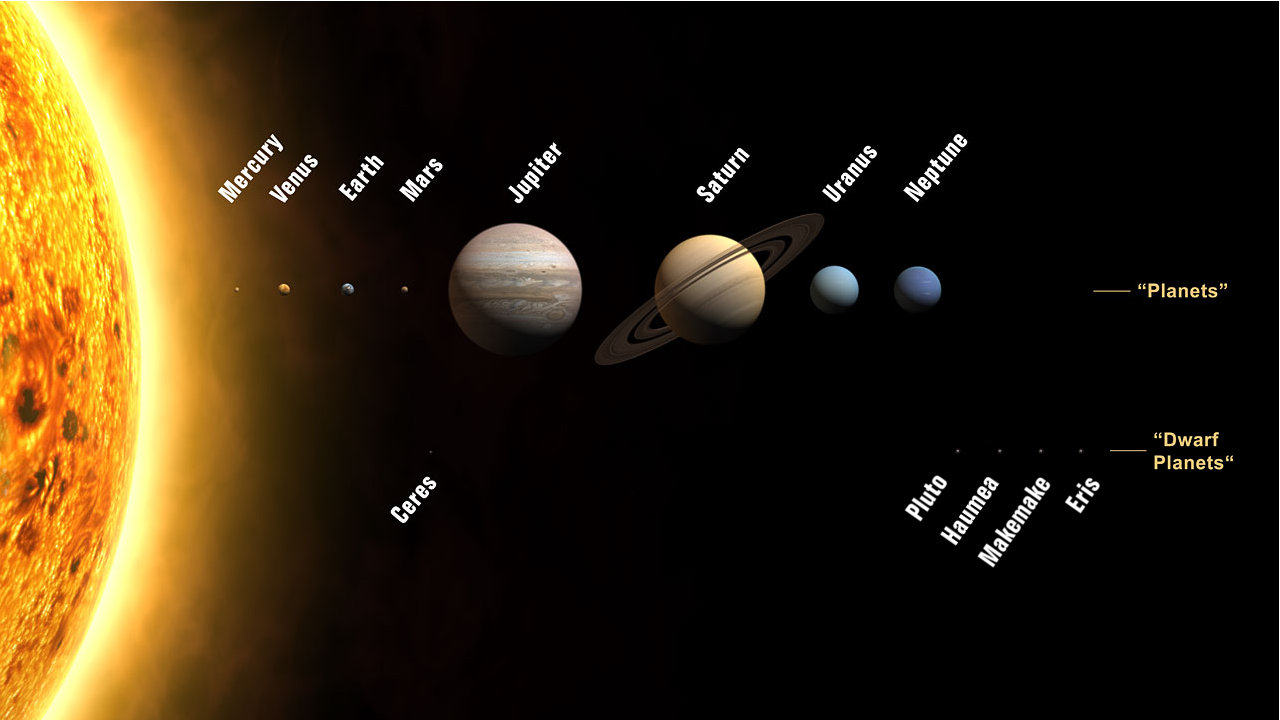
\includegraphics[width=0.75\textwidth]{image/Planets2008.jpg}
	\caption{Plants of Solar system}
    \label{fig:solar system}
\end{figure}
\footnote{Figure from \url{https://en.wikipedia.org/wiki/Solar_System}}

\section{Essential Codes and Functions Analysis}
For specific programs, we are extracted using samples of codes
\footnote{Prog6\_1\_sphere, Prog6\_2\_torus, Prog7\_1\_lightingADS and Prog9\_3\_environmentMapping respectively  } 
in textbook.
Furthermore, the running environment must to load \textbf{Modern OpenGL}
(vertex and fragment shaders), \textbf{GLEW},
\textbf{GLFW}, \textbf{GLM}, and \textbf{SOIL2 Library} in configuration.

\subsection{Model Object}
The main model objects to animate asters are sphere and torus
\footnote{The concrete class and functions also in Prog6\_1\_sphere, Prog6\_2\_torus} respectively.

\subsubsection{Sphere}\label{sec:sphere}
Firstly, we analysis the main ideas in \textbf{Sphere.cpp} in order to understand how to draw spheres 
by drawing inferences about other cases from one instance.

Some types of objects, such as spheres, torus, and so forth, have
mathematical definitions that lend themselves to algorithmic generation.
Consider for example a circle of radius R—coordinates of points around its
perimeter are well defined(Figure.\ref{fig:Rcoord}).
\begin{figure}[!htbp]
	\centering
	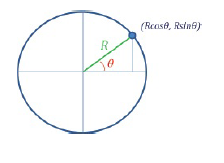
\includegraphics[width=0.75\textwidth]{image/R-coord.png}
	\caption{R—coordinates}
    \label{fig:Rcoord}
    \cite{alma991002986248905076}
\end{figure}

As the a circle of the coordinates, we can gain the strategy to get geometric sphere systematically.
\begin{enumerate}
    \item  
    Select a precision representing a number of circular \emph{horizontal slices}
through the sphere.\newline(Figure.\ref{fig:sphere1}) 
    \begin{figure}[!htbp]
        \centering
        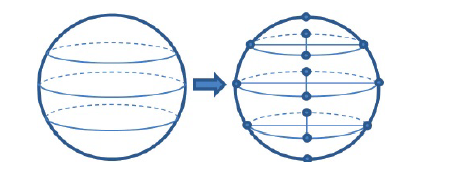
\includegraphics[width=0.75\textwidth]{image/sphere1.png}
        \caption{R—coordinates}
        \label{fig:sphere1}
        \cite{alma991002986248905076}
    \end{figure}
    \item 
    Subdivide the circumference of each circular slice into some number of
points according to the right side of Figure.\ref{fig:sphere1}. More points and horizontal slices
produces a more accurate and smoother model of the sphere. In our
model, each slice will have the same number of points.
    \item 
    We move along row of the vertices on the sphere in Figure.\ref{fig:sphere2} 
    to group the vertices into triangles. 
    \begin{figure}[!htbp]
        \centering
        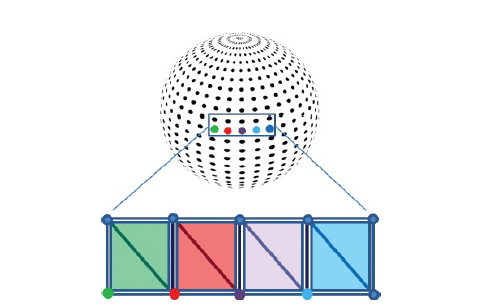
\includegraphics[width=0.75\textwidth]{image/sphere2.png}
        \caption{R—coordinates}
        \label{fig:sphere2}
        \cite{alma991002986248905076}
    \end{figure}
\end{enumerate}

Then we can then traverse the vertices in a circular fashion around each horizontal
slice, starting at the bottom of the sphere. We build two 
triangles forming a square region above and to its right, as shown earlier in
Figure.\ref{fig:sphere2}. 
The processing is organized into nested loops, as Figure.\ref{fig:vertices}.
    \begin{figure}[!htbp]
        \centering
        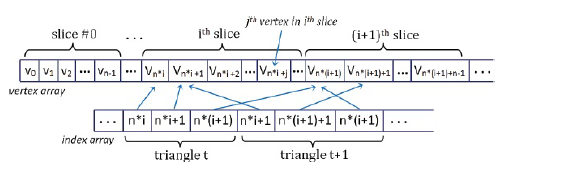
\includegraphics[width=0.75\textwidth]{image/vertices.png}
        \caption{Model Vertices}
        \label{fig:vertices}
        \cite{alma991002986248905076}
    \end{figure}

After getting geometry, the next point is to mapping the texture, which will be mentioned 
in \hyperref[sec:mapping]{Section.Texture Mapping}.

\subsubsection{Torus}
For the torus, 
We ues \textbf{Torus.cpp}, which is rather different from
what was done to build the sphere in \hyperref[sec:sphere]{\textbf{Sphere.cpp}} according to the algorithm which 
positions a vertex to the right of the origin and then rotates that vertex in a circle on the 
\textbf{XY} plane using a rotation around the \textbf{Z} axis to form a \emph{ring}. 
The ring is then moved outward by the \emph{inner radius} distance.
(Figure.\ref{fig:building toruss})
\begin{figure}[!htbp]
    \centering
    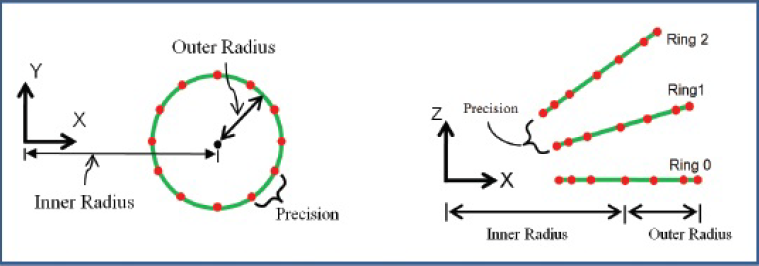
\includegraphics[width=0.75\textwidth]{image/building torus.png}
    \caption{Building Torus}
    \label{fig:building toruss}
    \cite{alma991002986248905076}
\end{figure}

To animate the ring of Saturn, the more difficult part is to regulate the parameters of ring,
including thickness. When we see the original model in source code
\footnote{Prog6\_2\_torus, Prog7\_1\_lightingADS}, the graphics is shown in Figure.\ref{fig:tor}.   
\begin{figure}[!htbp]
	\centering
	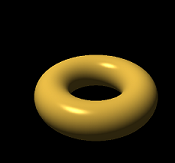
\includegraphics[width=0.75\textwidth]{image/torus.png}
	\caption{Model Torus}
    \label{fig:tor}
\end{figure}

Thus, by controlling corresponding functions(Code.\ref{code:ring}), we can get a model resembling a flat ring(Figure.\ref{fig:torring}). 
\label{code:ring}
\lstset{numbers=left,numberstyle=\tiny\color{gray}}
\lstinputlisting{code/ring.cpp}
\begin{figure}[!htbp]
	\centering
	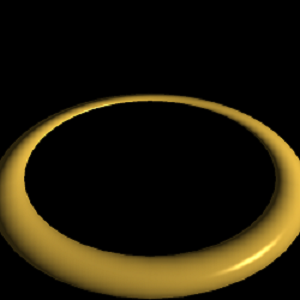
\includegraphics[width=0.75\textwidth]{image/torus ring.png}
	\caption{Model Ring}
    \label{fig:torring}
\end{figure}

\subsubsection{Matrix Stack}
For single object, we can easily call specific functions in different class, but we aim to use a 
kind of data structure to contain the multiply objects displaying in the whole window.
Therefore, we choose \emph{stack} in \textbf{C++ Standard Template Library (STL)} relatively
straightforward to adapt as a matrix stack.
An overview of how a \emph{display()} function using a matrix stack 
and the sequence of steps for the asters are typically organized in our textbook, so we may not repeat twice in report.

What we have changed compared with sample consists of scale, orbital position, inclination 
revolution and rotation. The specifically emphasizing points would be that 
the data of these characteristics is converted to parameters of functions in \textbf{GLM Library}
by calculating, but to give a friendly angle of view for audiences, the some orbital position of asters are adjusted factitiously. 
The Code.\ref{code:mvStack} which draws earth and moon shows how to realize.
\label{code:mvStack}
\lstset{numbers=left,numberstyle=\tiny\color{gray}}
\lstinputlisting{code/mvStack.cpp}


\subsection{Texture Mapping}\label{sec:mapping}
After the object is fully created, the next step is to map the texture to the object. 
To know which texture image is picked for certain mesh, there are points that represent mesh 
coordinates and the mesh texture image path file.

To have the texture wrapped in the object, first, the texture image must be called by
\emph{loadTexture} function from file \textbf{Utils.cpp} which is be encapsulated from \emph{SOIL\_load\_OGL\_texture} function of \textbf{OpenGL SOIL Library}. 
The sample of this function are provided in Code.\ref{code:loadTexture}. 
Then we are supposed to initialize textures of all asters in \emph{init()} function.
\label{code:loadTexture} 
\lstset{numbers=left,numberstyle=\tiny\color{gray}}
\lstinputlisting{code/loadTexture.cpp}  

Subsequently, the image can be assigned to a particular model or object. 
For the solar system project, the texture mapping process is quite easy because the texture image will only wrap the object. 
Then we add an uniform sampler variable(Code.\ref{code:uniform sampler variable}) declared in the shade to your set of uniforms.
\label{code:uniform sampler variable}
\lstset{numbers=left,numberstyle=\tiny\color{gray}}
\lstinputlisting{code/uniform.cpp}
The \emph{layout (binding=0)} portion of the declaration
specifies that this sampler is to be associated with texture unit 0.
A texture unit (and associated sampler) can be used to sample whichever
texture object you wish, and that can change at runtime. The \emph{display()} function
will need to specify which texture object you want the texture unit to sample for
the current frame. So each time drawing an object, we still need to activate a
texture unit and bind it to a particular texture object in Code.\ref{code:display}.
\label{code:display}
\lstset{numbers=left,numberstyle=\tiny\color{gray}}
\lstinputlisting{code/display.cpp}

Finally, the whole process of texture mapping can be abstracted as Figure.\ref{fig:how to texture}.
\begin{figure}[!htbp]
	\centering
	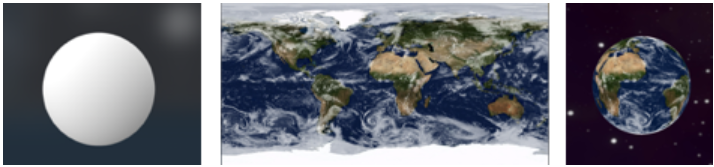
\includegraphics[width=0.75\textwidth]{image/how to texture.png}
	\caption{Texture Mapping}
    \label{fig:how to texture}
\end{figure}
\footnote{figure from \url{https://medium.com/@keynekassapa13/creating-the-solar-system-opengl-and-c-9d4e4798d759}}
% There are several custom parameters that need to be assigned to the texture configuration. 
% Wrapping configuration is related to how the texture image will be displayed when the coordinates are outside of the image range. 
% Filtering configuration is related to how the computer graphics handle the pixels when the image is being scaled or stretched.

\subsection{Camera}\label{sec:camera}
We use \textbf{W},\textbf{S},\textbf{A} and \textbf{D} in keyboard to adjust the 
position of camera by Code.\ref{code:camera}. 
And the original view of camera is on the position of sun, 
in other words, we just to control the position of sun.
And the operation of keyboard can be seen in Table.\ref{tab:keyboard}.
\label{code:camera}
\lstset{numbers=left,numberstyle=\tiny\color{gray}}
\lstinputlisting{code/camera.cpp}

\begin{table}[!hpbt]
    \centering
    \begin{tabular}{|c|c|}
    \hline
    W & translate forward \\ \hline
    S & translate backward \\ \hline   
    A & translate left  \\ \hline
    D & translate right\\ \hline                    
    \end{tabular}
    \caption{How to control keyboard}
    \label{tab:keyboard}
\end{table}

Then, in \emph{display(currentTime)} function we must pass the 
position parameters into \emph{vMat} and next set \emph{vLoc} 
which is a variable allocation for display according to Code.\ref{code:vnLoc}.
\label{code:vnLoc}
\lstset{numbers=left,numberstyle=\tiny\color{gray}}
\lstinputlisting{code/nLoc.cpp}


Finally, to apply camera in window we need \emph{key\_callback} function in Code.\ref{code:key}. Besides, 
in \emph{main()} function we need call \emph{glfwSetKeyCallback} to check whether the keyboard choosing 
\label{code:key}
\lstset{numbers=left,numberstyle=\tiny\color{gray}}
\lstinputlisting{code/key.cpp}


\subsection{Surface Lighting}
There are a number kinds of light to apply by \emph{.glsl} files in source code\footnote{Prog7\_1\_lightingADS},
and for this project we use \textbf{Position Light} initialization in \textbf{main.cpp}(Code.\ref{code:position light})
\label{code:position light}
\lstset{numbers=left,numberstyle=\tiny\color{gray}}
\lstinputlisting{code/light.cpp}

Subsequently, attenuation factors (Formula.\ref{equ:atten}) which can be modeled in a variety of ways,
have implication to \textbf{Position Light}. 
\begin{eqnarray}\label{equ:atten} 
    attenuation=\frac{1}{k_c+k_l*D+k_q*D^2}\quad(k_c\geqslant1,0\leqslant attenuation\leqslant1)\\
    \lim_{D\to \infty}attenuation=0
\end{eqnarray}
\footnote{$k_c$, $k_l$, $k_q$, and $D$ respectively refer to parameters for constant, linear, quadratic
attenuation and the distance from the light source.}

Then, the basic ADS computation that we need to perform is to determine the
reflection intensity ($I$) which includes \textbf{ambient}, \textbf{diffuse} and \textbf{specular} for each pixel(Figure.\ref{fig:ASD}). 
This computation takes the following Formula.\ref{equ:ligObser}.
\begin{equation}\label{equ:ligObser} 
    I_{observed}=I_{ambient}+I_{diffuse}+I_{specular}
\end{equation}
\begin{figure}[!htbp]
	\centering
	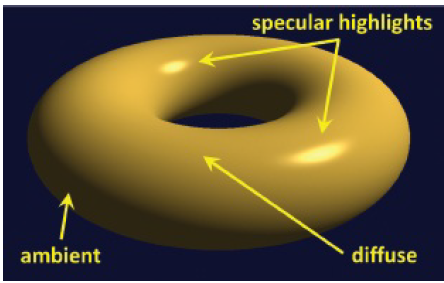
\includegraphics[width=0.75\textwidth]{image/ASD.png}
	\caption{ADS Lighting Contributions}
    \label{fig:ASD}
    \cite{alma991002986248905076}
\end{figure}

Ambient contribution is the product of the specified ambient
light and the specified ambient coefficient of the material(Formula.\ref{equ:ligAmb}).
\begin{equation}\label{equ:ligAmb} 
    I_{ambient}=k_a*Light_{ambient}
\end{equation}\footnote{$k_a$ refer to \textbf{Ambient Radiation Coefficient} of materials} 

For diffuse contribution, it is more complex because it depends on the angle of
incidence between the light and the surface(Figure.\ref{fig:angle of lighting1}) to get Formula.\ref{equ:ligDif1}.
\begin{figure}[!htbp]
	\centering
	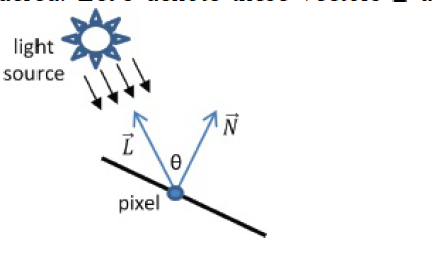
\includegraphics[width=0.75\textwidth]{image/angle of lighting1.png}
	\caption{Angle of Light Incidence}
    \label{fig:angle of lighting1}
    \cite{alma991002986248905076}
\end{figure}
\begin{equation}\label{equ:ligDif1} 
    I_{diffuse}=k_d*Light_{diffuse}*\cos(\theta)
\end{equation}\footnote{$k_d$ refer to \textbf{Diffuse Radiation Coefficient} of materials}
And Formula.\ref{equ:ligDif1} can be deducted to Formula.\ref{equ:ligDif2}.
\begin{equation}\label{equ:ligDif2} 
    I_{diffuse}=k_d*Light_{diffuse}*\max((\overrightarrow{N}\bullet\overrightarrow{L}),0) 
\end{equation}

Specular contribution determines whether the pixel being rendered should be
brightened because it is part of a \textbf{specular highlight}. It involves not only the
angle of incidence of the light source, but also the angle between the reflection
of the light on the surface and the viewing angle of the eye relative to the
object’s surface(Figure.\ref{fig:angle of lighting2}). So the we calculate it by Formula.\ref{equ:ligSpe}.
\begin{equation}\label{equ:ligSpe} 
    I_{specular}=k_s*Light_{specular}*\max((\overrightarrow{N}\bullet\overrightarrow{L})^n,0)
\end{equation}\footnote{$k_s$ refer to \textbf{Specular Radiation Coefficient} of materials} 
\begin{figure}[!htbp]
	\centering
	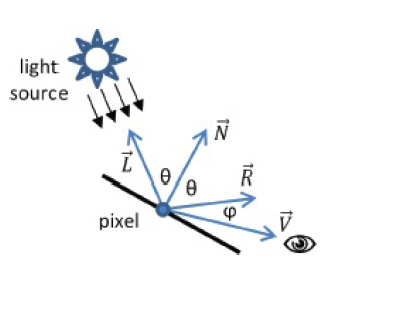
\includegraphics[width=0.75\textwidth]{image/angle of lighting2.png}
	\caption{View Angle Incidence}
    \label{fig:angle of lighting2}
    \cite{alma991002986248905076}
\end{figure}

Finally, we combine surface texture and light to the asters except sun according to Formula.\ref{equ:colFrag}.
Because sun is the position of light without adding shade to make it dark.   
\begin{equation}\label{equ:colFrag} 
    C_{frag}=C_{texture}*(I_{ambient}+I_{diffuse}+I_{specular})
\end{equation}\footnote{$C$ refer to color}
We can easily add the code(Code.\ref{code:frag}) in \emph{fraghShade.glsl} to realize the aim.  
\label{code:frag}
\lstset{numbers=left,numberstyle=\tiny\color{gray}}
\lstinputlisting{code/frag.cpp}

\subsection{Sky cube Mapping}
To mapping the texture to the whole background, it is simple to create cube model in 3D to 
achieve this aim which is similar to the contents of Section.\hyperref[sec:mapping]{Texture Mapping}.
Firstly, we initiate the vertices of cube model 
by \emph{float cubeVertexPositions[108]} in \emph{setupVertices()} function.
Then we add codes in \emph{init()} function, but we use \emph{loadCubeMap()} function from \textbf{Utils.cpp}
in order to load texture on six sides of cube in Code.\ref{code:cubemap}. 
\label{code:cubemap}
\lstset{numbers=left,numberstyle=\tiny\color{gray}}
\lstinputlisting{code/cubemap.cpp}

%glFrontFace(GL_CCW);	// cube is CW, but we are viewing the inside

Because we add lighting in \textbf{vertShader.glsl} and \textbf{fragShader.glsl}, 
we need create new files of shade--\textbf{vertCubeShader.glsl} and \textbf{fragCubeShader.glsl} 
realization of sky cube. 

\section{Output and Program Test} 
When running the program, the view of camera is on the position of sun 
which can only see the asters surround,  
so we need to press down \textbf{S} in keyboard to put camera far form the origin. 
After that we repeat adjust to find different angle to observe the solar system model. 
And the output in window can be seen in Figure.\ref{fig:run sample}. 
(Specific way to use keyboard to control camera can be review in Section.\hyperref[sec:camera]{Camera}) 
\begin{figure}[!htbp]
	\centering
	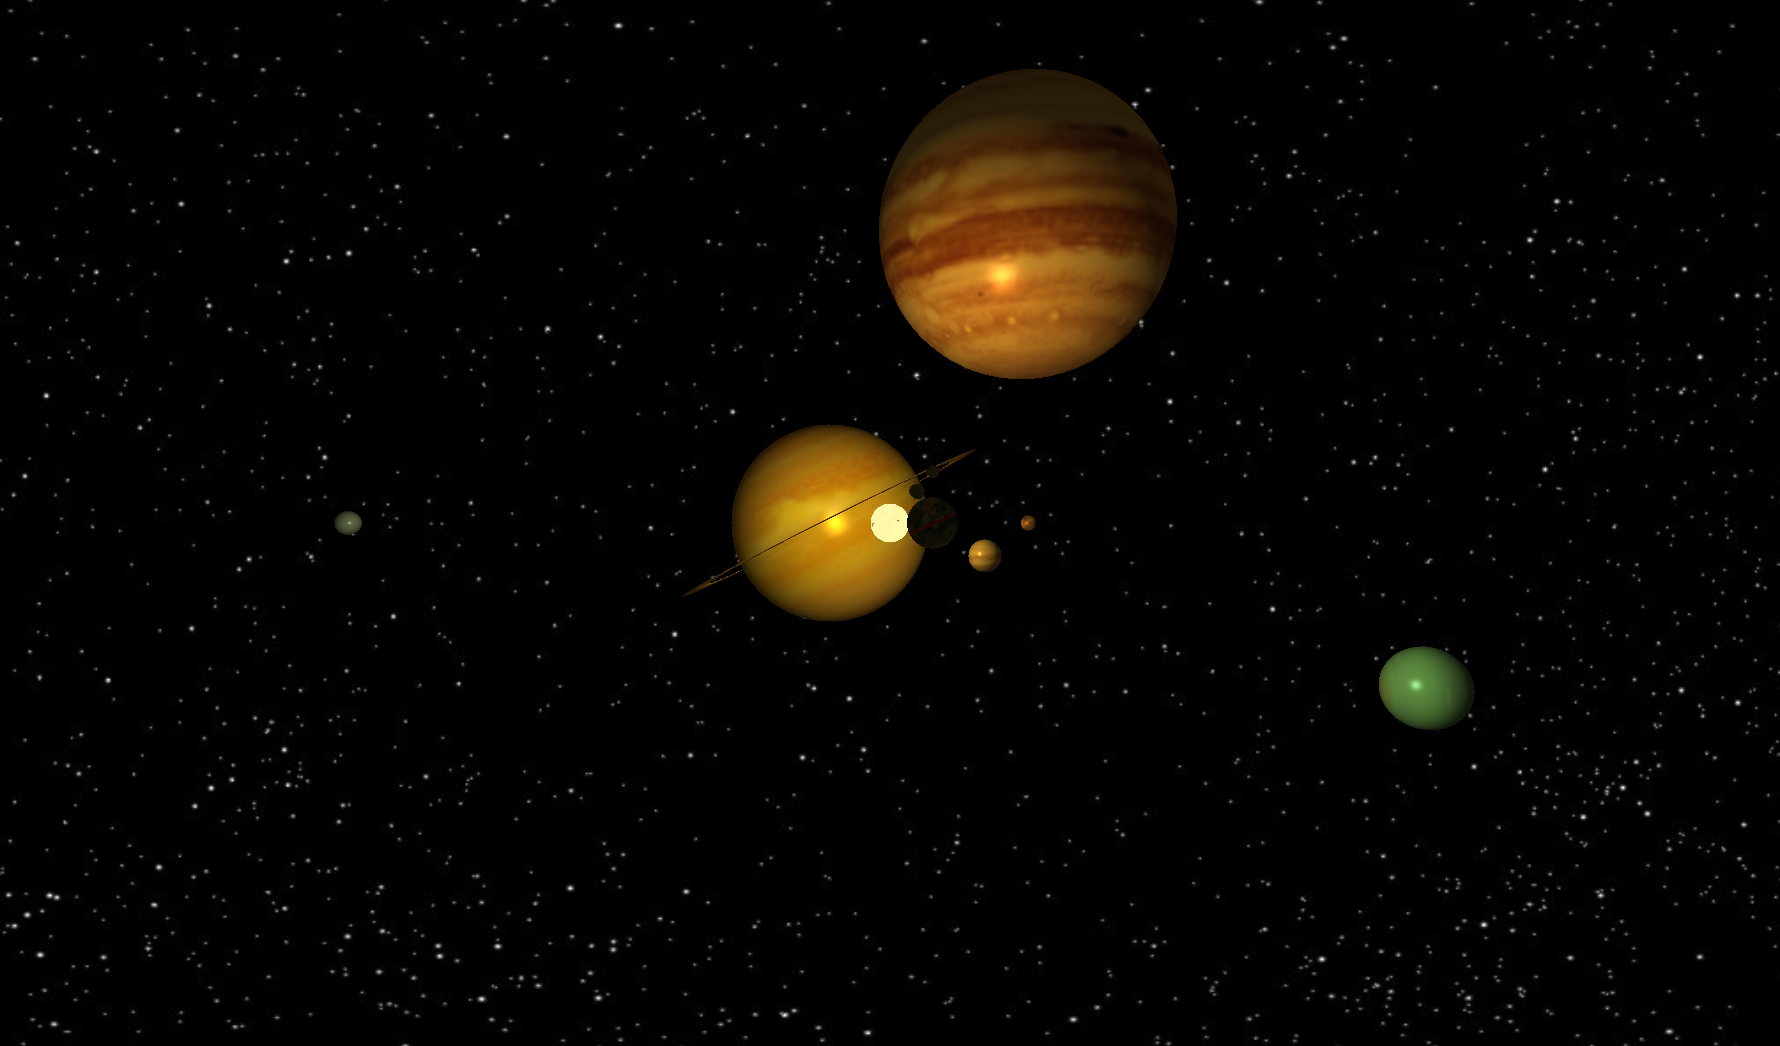
\includegraphics[width=0.75\textwidth]{image/run sample.png}
	\caption{Sample of Output}
    \label{fig:run sample}
\end{figure}
\section{Summary}
Through this experiment, we learned and mastered 
how to transformations, texture mapping, lighting and
window event handling and realized the region filling. 
We also know that graphics programming has a reputation for being among the most challenging
computer science topics to learn. 
In the process of compiling the algorithm by pushing and popping stack repeatably, 
we constantly improve the composition of a picture and solve the difficulties with the help of classmate.
However, there are still some improved effective function which has not been written and implemented, 
and the program is constantly optimized in the continuous improvement, 



\bibliographystyle{plain}
\bibliography{ref.bib}

\end{document}